\documentclass{article}
% Change "article" to "report" to get rid of page number on title page
\usepackage{amsmath,amsfonts,amsthm,amssymb}
\usepackage{setspace}
\usepackage{fancyhdr}
\usepackage{lastpage}
\usepackage{extramarks}
\usepackage{chngpage}
\usepackage{soul}
\usepackage[usenames,dvipsnames]{color}
\usepackage{graphicx,float,wrapfig}
\usepackage{ifthen}
\usepackage{listings}
\usepackage{courier}
\usepackage{subcaption}
\usepackage{braket}
\usepackage{amsmath}
\DeclareMathOperator{\Tr}{Tr}

%   !!!!!!!!!!!!!!!!!!!!!!!!!!!!!!!!!!!!!!!!!!!!!!!!!!!!!
%
%   Here put your info (name, due date, title etc).
%   the rest should be left unchanged.
%
%
%
%   !!!!!!!!!!!!!!!!!!!!!!!!!!!!!!!!!!!!!!!!!!!!!!!!!!!!!


% Homework Specific Information
\newcommand{\hmwkTitle}{}
\newcommand{\hmwkSubTitle}{Steepest descent, conjugate gradients and SVD}
\newcommand{\hmwkDueDate}{June 08, 2023}
\newcommand{\hmwkClass}{Computational Physics III}
\newcommand{\hmwkClassTime}{}
%\newcommand{\hmwkClassInstructor}{Prof. Oleg Yazyev}
\newcommand{\hmwkAuthorName}{Salomon Guinchard}
\newcommand{\beq}{\begin{equation}}
\newcommand{\eeq}{\end{equation}}
\graphicspath{{./Illustrations/}{./IllustrationsResults/}}  
\newcommand{\bx}{\mathbf{x}}
\newcommand{\bA}{\mathbf{A}}
\newcommand{\bb}{\mathbf{b}}
%
%


% In case you need to adjust margins:
\topmargin=-0.45in      %
\evensidemargin=0in     %
\oddsidemargin=0in      %
\textwidth=6.5in        %
\textheight=9.5in       %
\headsep=0.25in         %

% This is the color used for  comments below
\definecolor{MyDarkGreen}{rgb}{0.0,0.4,0.0}

% For faster processing, load Matlab syntax for listings
\lstloadlanguages{Matlab}%
\lstset{language=Matlab,                        % Use MATLAB
        frame=single,                           % Single frame around code
        basicstyle=\small\ttfamily,             % Use small true type font
        keywordstyle=[1]\color{Blue}\bf,        % MATLAB functions bold and blue
        keywordstyle=[2]\color{Purple},         % MATLAB function arguments purple
        keywordstyle=[3]\color{Blue}\underbar,  % User functions underlined and blue
        identifierstyle=,                       % Nothing special about identifiers
                                                % Comments small dark green courier
        commentstyle=\usefont{T1}{pcr}{m}{sl}\color{MyDarkGreen}\small,
        stringstyle=\color{Purple},             % Strings are purple
        showstringspaces=false,                 % Don't put marks in string spaces
        tabsize=3,                              % 5 spaces per tab
        %
        %%% Put standard MATLAB functions not included in the default
        %%% language here
        morekeywords={xlim,ylim,var,alpha,factorial,poissrnd,normpdf,normcdf},
        %
        %%% Put MATLAB function parameters here
        morekeywords=[2]{on, off, interp},
        %
        %%% Put user defined functions here
        morekeywords=[3]{FindESS, homework_example},
        %
        morecomment=[l][\color{Blue}]{...},     % Line continuation (...) like blue comment
        numbers=left,                           % Line numbers on left
        firstnumber=1,                          % Line numbers start with line 1
        numberstyle=\tiny\color{Blue},          % Line numbers are blue
        stepnumber=1                        % Line numbers go in steps of 5
        }

% Setup the header and footer
\pagestyle{fancy}                                                       %
\lhead{\hmwkAuthorName}                                                 %
%\chead{\hmwkClass\ (\hmwkClassInstructor\ \hmwkClassTime): \hmwkTitle}  %
\rhead{\hmwkClass\ : \hmwkTitle}  %
%\rhead{\firstxmark}                                                     %
\lfoot{\lastxmark}                                                      %
\cfoot{}                                                                %
\rfoot{Page\ \thepage\ of\ \protect\pageref{LastPage}}                  %
\renewcommand\headrulewidth{0.4pt}                                      %
\renewcommand\footrulewidth{0.4pt}                                      %

% This is used to trace down (pin point) problems
% in latexing a document:
%\tracingall

%%%%%%%%%%%%%%%%%%%%%%%%%%%%%%%%%%%%%%%%%%%%%%%%%%%%%%%%%%%%%
% Some tools
\newcommand{\enterProblemHeader}[1]{\nobreak\extramarks{#1}{#1 continued on next page\ldots}\nobreak%
                                    \nobreak\extramarks{#1 (continued)}{#1 continued on next page\ldots}\nobreak}%
\newcommand{\exitProblemHeader}[1]{\nobreak\extramarks{#1 (continued)}{#1 continued on next page\ldots}\nobreak%
                                   \nobreak\extramarks{#1}{}\nobreak}%

\newlength{\labelLength}
\newcommand{\labelAnswer}[2]
  {\settowidth{\labelLength}{#1}%
   \addtolength{\labelLength}{0.25in}%
   \changetext{}{-\labelLength}{}{}{}%
   \noindent\fbox{\begin{minipage}[c]{\columnwidth}#2\end{minipage}}%
   \marginpar{\fbox{#1}}%

   % We put the blank space above in order to make sure this
   % \marginpar gets correctly placed.
   \changetext{}{+\labelLength}{}{}{}}%

\setcounter{secnumdepth}{0}
\newcommand{\homeworkProblemName}{}%
\newcounter{homeworkProblemCounter}%
\newenvironment{homeworkProblem}[1][Problem \arabic{homeworkProblemCounter}]%
  {\stepcounter{homeworkProblemCounter}%
   \renewcommand{\homeworkProblemName}{#1}%
   \section{\homeworkProblemName}%
   \enterProblemHeader{\homeworkProblemName}}%
  {\exitProblemHeader{\homeworkProblemName}}%

\newcommand{\problemAnswer}[1]
  {\noindent\fbox{\begin{minipage}[c]{\columnwidth}#1\end{minipage}}}%

\newcommand{\problemLAnswer}[1]
  {\labelAnswer{\homeworkProblemName}{#1}}

\newcommand{\homeworkSectionName}{}%
\newlength{\homeworkSectionLabelLength}{}%
\newenvironment{homeworkSection}[1]%
  {% We put this space here to make sure we're not connected to the above.
   % Otherwise the changetext can do funny things to the other margin

   \renewcommand{\homeworkSectionName}{#1}%
   \settowidth{\homeworkSectionLabelLength}{\homeworkSectionName}%
   \addtolength{\homeworkSectionLabelLength}{0.25in}%
   %\changetext{}{-\homeworkSectionLabelLength}{}{}{}%
   \subsection{\homeworkSectionName}%
   \enterProblemHeader{\homeworkProblemName\ [\homeworkSectionName]}}%
  {\enterProblemHeader{\homeworkProblemName}%

   % We put the blank space above in order to make sure this margin
   % change doesn't happen too soon (otherwise \sectionAnswer's can
   % get ugly about their \marginpar placement.
  % \changetext{}{+\homeworkSectionLabelLength}{}{}{}
   }%

\newcommand{\sectionAnswer}[1]
  {% We put this space here to make sure we're disconnected from the previous
   % passage

   \noindent\fbox{\begin{minipage}[c]{\columnwidth}#1\end{minipage}}%
   \enterProblemHeader{\homeworkProblemName}\exitProblemHeader{\homeworkProblemName}%
   \marginpar{\fbox{\homeworkSectionName}}%

   % We put the blank space above in order to make sure this
   % \marginpar gets correctly placed.
   }%

%%% I think \captionwidth (commented out below) can go away
%%%
%% Edits the caption width
%\newcommand{\captionwidth}[1]{%
%  \dimen0=\columnwidth   \advance\dimen0 by-#1\relax
%  \divide\dimen0 by2
%  \advance\leftskip by\dimen0
%  \advance\rightskip by\dimen0
%}

% Includes a figure
% The first parameter is the label, which is also the name of the figure
%   with or without the extension (e.g., .eps, .fig, .png, .gif, etc.)
%   IF NO EXTENSION IS GIVEN, LaTeX will look for the most appropriate one.
%   This means that if a DVI (or PS) is being produced, it will look for
%   an eps. If a PDF is being produced, it will look for nearly anything
%   else (gif, jpg, png, et cetera). Because of this, when I generate figures
%   I typically generate an eps and a png to allow me the most flexibility
%   when rendering my document.
% The second parameter is the width of the figure normalized to column width
%   (e.g. 0.5 for half a column, 0.75 for 75% of the column)
% The third parameter is the caption.
\newcommand{\scalefig}[3]{
  \begin{figure}[ht!]
    % Requires \usepackage{graphicx}
    \centering
    \includegraphics[width=#2\columnwidth]{#1}
    %%% I think \captionwidth (see above) can go away as long as
    %%% \centering is above
    %\captionwidth{#2\columnwidth}%
    \caption{#3}
    \label{#1}
  \end{figure}}

% Includes a MATLAB script.
% The first parameter is the label, which also is the name of the script
%   without the .m.
% The second parameter is the optional caption.
\newcommand{\matlabscript}[2]
  {\begin{itemize}\item[]\lstinputlisting[caption=#2,label=#1]{#1.m}\end{itemize}}

%%%%%%%%%%%%%%%%%%%%%%%%%%%%%%%%%%%%%%%%%%%%%%%%%%%%%%%%%%%%%


%%%%%%%%%%%%%%%%%%%%%%%%%%%%%%%%%%%%%%%%%%%%%%%%%%%%%%%%%%%%%
% Make title
%\title{\vspace{2in}\textmd{\textbf{\hmwkClass:\ \hmwkTitle\ifthenelse{\equal{\hmwkSubTitle}{}}{}{\\\hmwkSubTitle}}}\\\normalsize\vspace{0.1in}\small{Due\ on\ \hmwkDueDate}\\\vspace{0.1in}\large{\textit{\hmwkClassInstructor\ \hmwkClassTime}}\vspace{3in}}
\title{\vspace{2in}\textmd{\textbf{\hmwkClass:\ \hmwkTitle\ifthenelse{\equal{\hmwkSubTitle}{}}{}{\\\hmwkSubTitle}}}\\\normalsize\vspace{0.1in}\small{Due\ on\ \hmwkDueDate}\\\vspace{0.1in}\large{\textit{ \hmwkClassTime}}\vspace{3in}}
\date{}
\author{\textbf{\hmwkAuthorName}}
%%%%%%%%%%%%%%%%%%%%%%%%%%%%%%%%%%%%%%%%%%%%%%%%%%%%%%%%%%%%%

\begin{document}
\begin{spacing}{1.1}
\maketitle
% Uncomment the \tableofcontents and \newpage lines to get a Contents page
% Uncomment the \setcounter line as well if you do NOT want subsections
%       listed in Contents
%\setcounter{tocdepth}{1}
\newpage
\tableofcontents
\newpage

% When problems are long, it may be desirable to put a \newpage or a
% \clearpage before each homeworkProblem environmenthttps://www.overleaf.com/project/5e6b2eb0146d4b00014629ac

\newpage

\begin{homeworkProblem}

\section{Steepest descent and conjugate gradient}

Say one has the following linear system of equations to solve:\\

\beq
\mathbf{A} \mathbf{x} = \mathbf{b},\label{lin_syst}
\eeq\\

\noindent where $\mathbf{A} $ is square, symmetric and positive definite, and $\mathbf{x}$, $\mathbf{b}$ are column vectors. Then two algorithms can be used to solve the linear system from Eq.(\ref{lin_syst}), namely the steepest descent (SD) and the conjugate gradient (CG) methods. Both methods exploit the fact that solving Eq.(\ref{lin_syst}) for $\mathbf{x}$ is equivalent to extremizing the following quadratic form $\mathbf{f}$: \\

\beq
\mathbf{f}(\mathbf{x}) = \mathbf{x}^T\mathbf{A} \mathbf{x} -\mathbf{b}^T \mathbf{x} + \mathbf{c},\label{quad_form}
\eeq\\

\noindent for an arbitrary constant $\mathbf{c}$ since the gradient of $\mathbf{f}$ that we shall denote by $\mathbf{f}'$ recovers Eq.(\ref{lin_syst}):\\

\beq
\mathbf{f}'(\mathbf{x}) = \mathbf{A} \mathbf{x} - \mathbf{b}.
\eeq\\

\noindent Thus, one notices that finding the values of $\mathbf{x}$ that extremize $\mathbf{f}$ is equivalent to finding the zeros of the gradient and solving Eq.(\ref{lin_syst}).\\

\begin{homeworkSection}{(1) Algorithms} 
	

The \textbf{SD} method starts from an arbitrary $\bx^{(0)}$ such that each step of the algorithm gives a point $\bx^{(i)}$ closer to the solution $\bx$. At each step, the direction of the steepest descent of the quadratic form from Eq.(\ref{quad_form}) is found and the minimum along this direction is determined, leading to the point $\bx^{(i+1)}$. Hence the resulting sequence $\{ \bx^{(i)}\}  $ is decreasing and the convergence rate of the error to the solution $\mathbf{e}^{(i)} :=\bx^{(i)}-\bx$ follows:\\

\beq
\frac{|\mathbf{e}^{(i)}|_{\bA}}{|\mathbf{e}^{(0)}|_{\bA}} \leq \Bigg(\frac{\kappa-1}{\kappa+1}\Bigg)^{i},\label{rel_SD}
\eeq\\

\noindent where $|\bx |_{\bA} :=(\bx^{T}\bA\bx)^{1/2}$ and $\kappa$ is the so called condition number of $\bA$, that is the ratio of the largest singular value of $\bA$ to the lowest.\\

 
The \textbf{CG} method shares basically the same base, the only difference is that the vectors from each step are no longer orthogonal to each other, but $\bA$-orthogonal, that is $\bx \cdot \mathbf{y} = \bx^T \bA \mathbf{y}$. This condition turns out to be very efficient, in the sense that if one were to consider an ideal case without numerical imprecision, the algorithme should converge in $n$ steps, with $n$ the size of the matrix. The relative error follows Eq.(\ref{rel_CG}).

\beq 
\frac{|\mathbf{e}^{(i)}|_{\bA}}{|\mathbf{e}^{(0)}|_{\bA}}\le  \Bigg(\frac{\sqrt{\kappa}-1}{\sqrt{\kappa}+1}\Bigg)^{i}\label{rel_CG}
\eeq  \\


\noindent The two algorithms have been implemented in the following scripts and the tests were passed successfully.\\

\matlabscript{simple}{Matlab script for the steepest descent method}

\matlabscript{simple2}{Matlab script for the conjugate gradient method}

\end{homeworkSection}

\begin{homeworkSection}{(2) System solving}

Using the matrices $\bA_i$ and the vectors $\mathbf{b}_i$ $i=1,2$ from the file \verb|Matrices.mat|, let us now use the previous algorithms to solve the system from Eq.(\ref{lin_syst}), and plot the relative error to the exact solution at each iteration. Fig.(\ref{N=5_fig}) and Fig.(\ref{N=50_fig}) show respectively the relative error at each iteration for both the steepest descent and the conjugate gradient methods for two distinct sizes for the matrice $\bA$: $N=5$ and $N=50$.\\

\newpage

\begin{figure}[h!]
\centering
	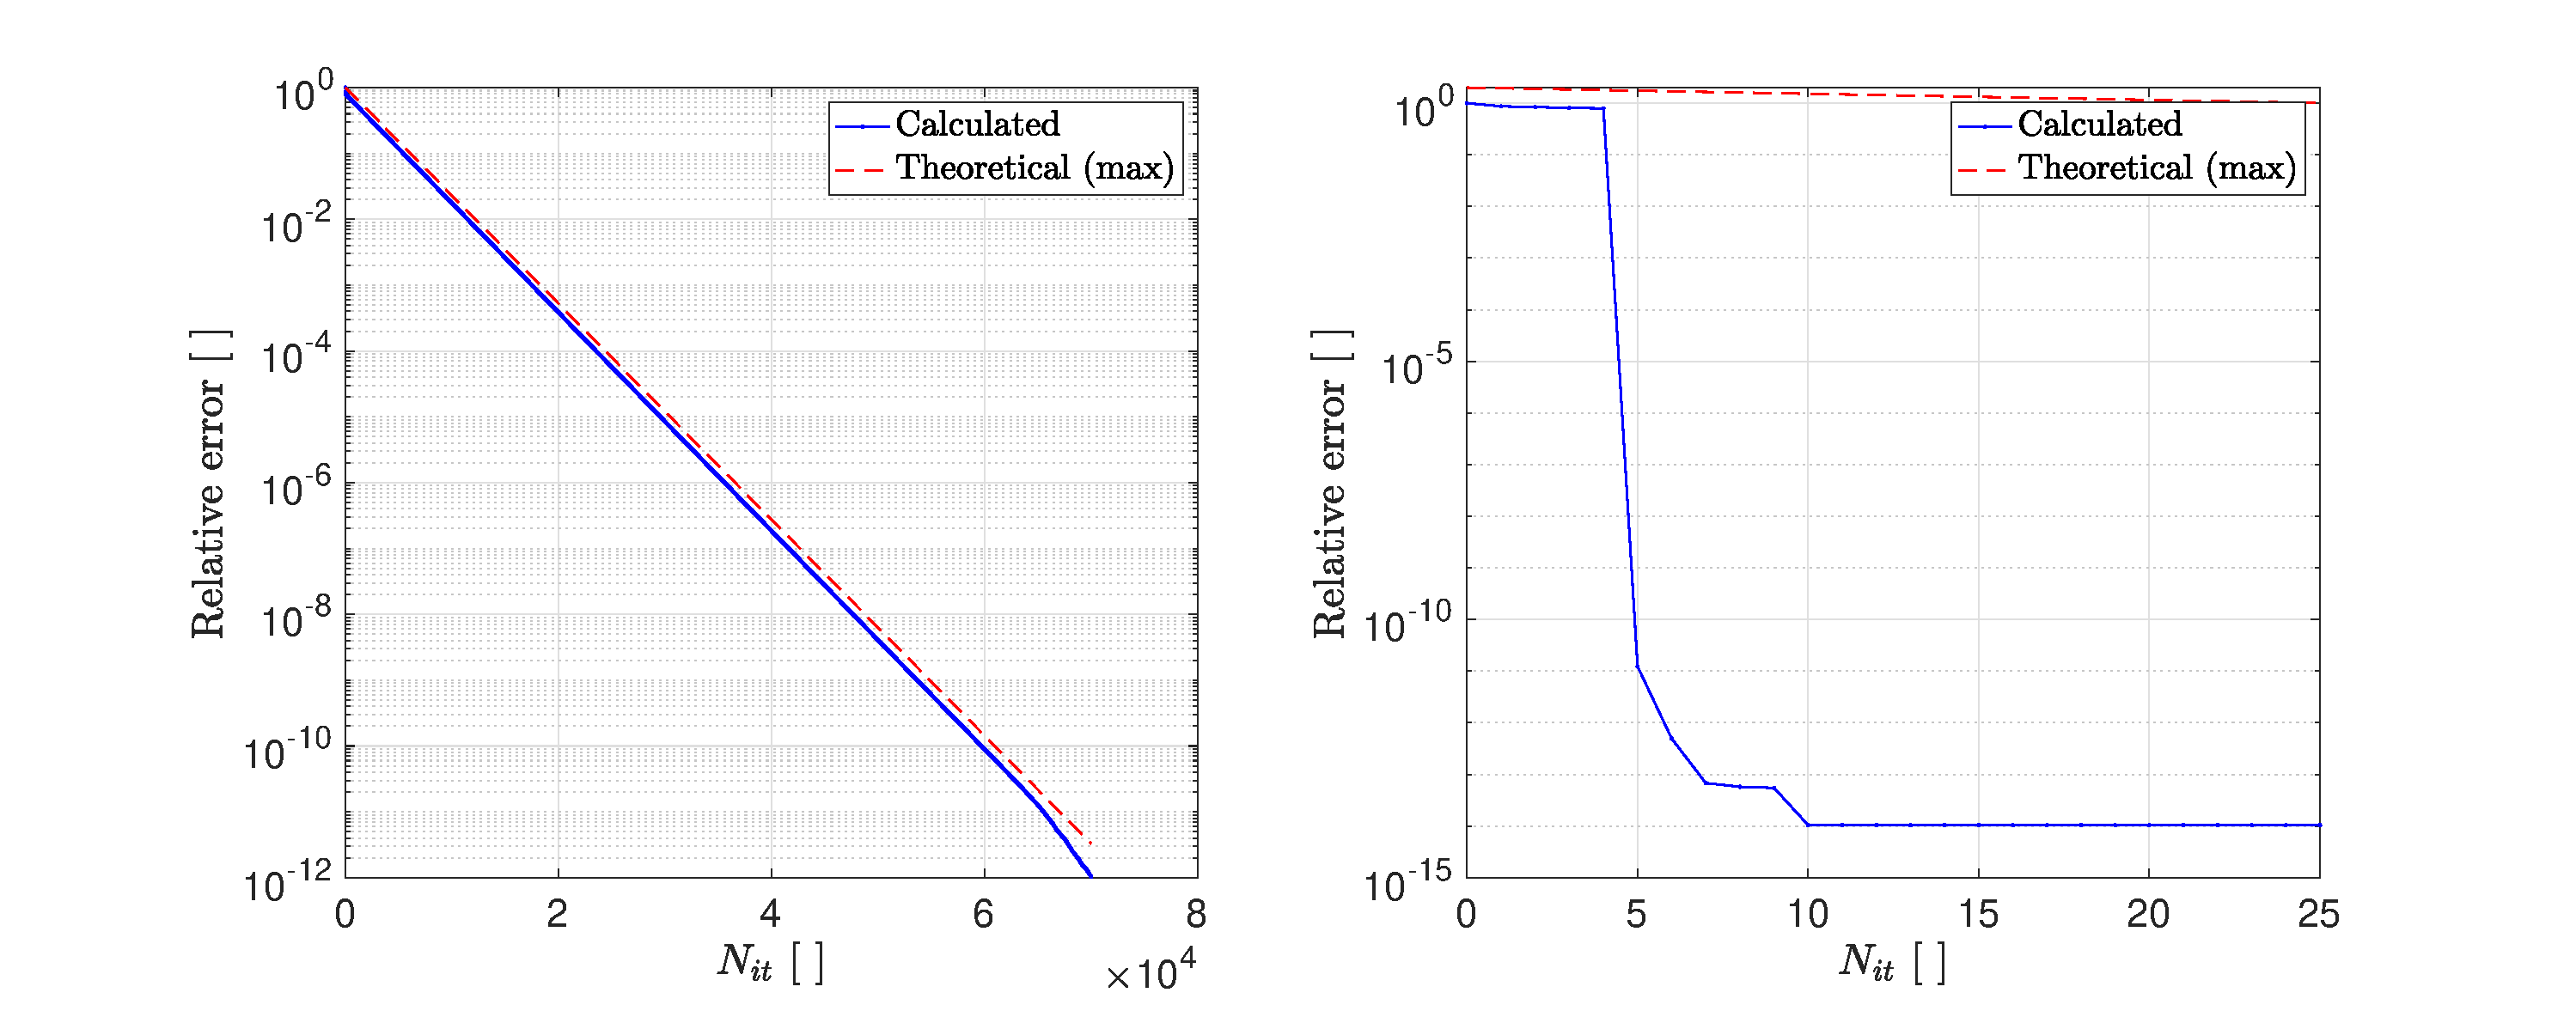
\includegraphics[width = 1 \textwidth]{N=5.eps}
	\caption{\label{N=5_fig}  Left: Relative error for $N=5$ and the steepest descent method, as a function of the number of iterations - Right: Same for the conjugate gradient method}
\end{figure} 

\begin{figure}[h!]
\centering
	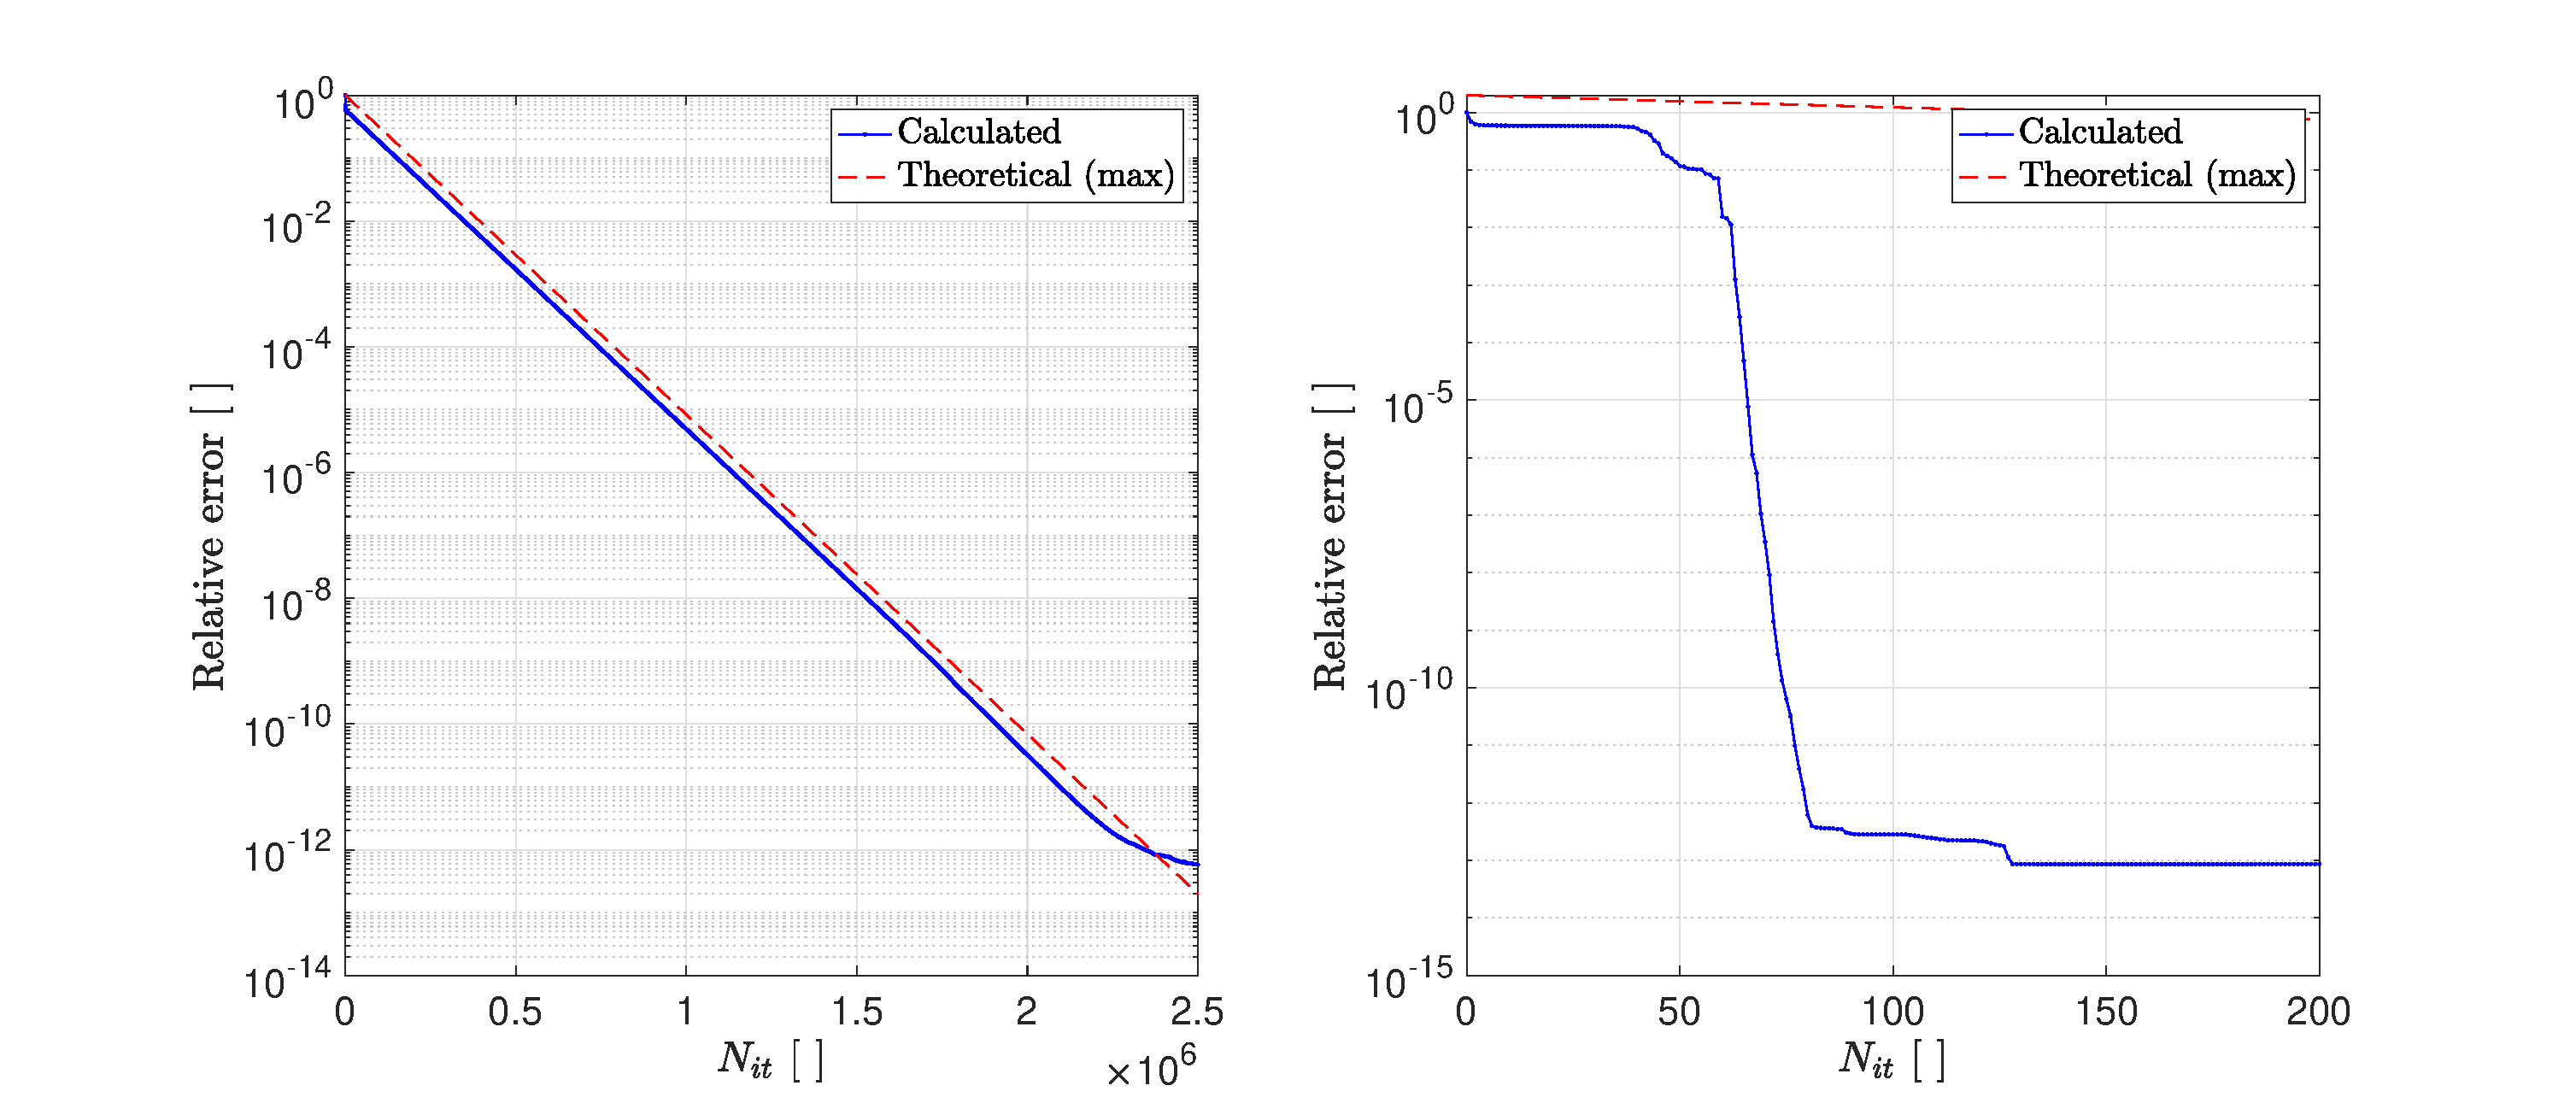
\includegraphics[width = 1 \textwidth]{N=50.eps}
	\caption{\label{N=50_fig}   Left: Relative error for $N=50$ and the steepest descent method as a function of the number of iterations - Right: Same for the conjugate gradient method}
\end{figure} 


\end{homeworkSection}

\begin{homeworkSection}{(3) Convergence and machine precision tolerance} 

In the two cases studied previously, with $N=5$ and $N=50$, one notes that the conjugate gradient method converges much faster towards the solution than the steepest descent method. Indeed, in the case $N=5$, the SD method needs about $7\cdot 10^4$ iterations to converge whereas the CG needs only 10 iterations. In the case $N=50$, $\sim2.4\cdot 10^6$ iterations were needed for the SD to converge against $\sim 130$ for the CG. In fact, it is possible to obtain a theoretical approximate maximum for the minimum of iterations required to achieve a relative error of the order of the machine precision $\epsilon$. It suffices to invert the relation from Eq.(\ref{rel_CG}) and Eq.(\ref{rel_SD}), yielding the expression  $N_{it}^{\epsilon} = \ln(\epsilon)/\ln((\kappa-1)/(\kappa+1))$ for the SD method, where $\kappa$ is the condition number of the matrix. Hence, in the case of $N=5$ (SD), one gets that $N_{it}^{\epsilon} = 95421 \sim 9\cdot 10^4$ and for $N=50$, $N_{it}^{\epsilon} = 3081446 \sim 3\cdot 10^6$ which are compatible results with those observed on Fig.(\ref{N=5_fig}) and Fig.(\ref{N=50_fig}).\\
	
\end{homeworkSection}

\vspace{1cm}



\end{homeworkProblem}

%%%%%%%%%%%%%%%%%%%%%%%%%%%%%%%%%%%%%%%%%%%%%%%%
%%%%%%%%%%%%%%%%%%%%%%%%%%%%%%%%%%%%%%%%%%%%%%%%
\newpage

\begin{homeworkProblem}

\section{Discretization of Poisson Equation}

Let us define the following system, consisting in a square grid of size $L\times L$ with $L=45$. Let  a charge $Q=1$C at the center of the grid. Two electrodes of length $L/3$, each kept at the  potential of $V_0=1$V are disposed (and centered) on the left and right sides. The remaining boundary is insulated, that is no electric field $ \mathbf{E}=\nabla V$ perpendicular to the boundary is present elsewhere. Recall that if the medium is devoid of magnetic field or electrical current, the electric potential $V(x,y)$ satisfies Poisson's equation:\\

\begin{gather}\label{poisson}
    \Delta V(x,y)=-\frac{\rho(x,y)}{\epsilon}
\end{gather}\\

The electric potential resulting from that test charge and the electrodes, setting $\epsilon=1$, will now be determined using the SD and CG methods derived previously.\\

\begin{homeworkSection}{(1) Discretization} 

To study the system and solve Poisson's equation, one has to discretize the problem so that it can be recast in the form of a system of linear equations $\bA A\bx=\mathbf{b}$. To do so, a grid of size $N\times N$ is considered, with $N=45$. Therefore, the discretized system is composed of $N^2$ points $(x_i,y_j)$. Let us now apply the following change of coordinates $(x_i,y_j)\rightarrow r_k$, $k\in\{1,N^2\}$ so the discretisation of the Laplacian operator is easier. Thus the matrix $\bA$ now becomes a matrix of size $N^2\times N^2$, and $\bx$ takes the following form $\bx=(V_1,...,V_{N^2})^T$. Moreoever, the Laplacian operator has been discretized using second order finite differences:\\

\begin{gather}\label{laplacian}              
   \nabla^2V(r_k)\approx\frac{V_{k+1}+V_{k-1}+V_{k+N}+V_{k-N}-4V_{k}}{h^2}
\end{gather}\\

where $V_k\equiv V(r_k)$ and $h$ is the mesh parameter, that is the distance between to neighboring points on the grid. Note that Eq.(\ref{laplacian}) only holds for the interior of the system, and not on the boundary. Indeed, take for example the left edge of the system, without considering the corners, which have to be treated separately. In that case, the discretized Laplacian becomes:\\

\begin{gather}
    \nabla^2V(r_k)\approx\frac{V_{k+1}+V_{k+N}+V_{k-N}-4V_{k}}{h^2}
\end{gather}\\


The same reasoning holds for the other edges of the system, as well as for the 4 corners. Now, let us focus on the implementation of the boundary conditions (BC). First, let us recall that the matrix $\bA$ is assumed to be symmetric and positive definite, since the SD and CG algorithms will be used to solve the system. Therefore, implementing the BC in the matrix $\bA$ would break the symmetry required by the SD and CG methods. This constraint can however be respected by transferring the BC into the right-hand side of the Poisson equation, i.e. into the charge density term $\rho$ (see Eq.(\ref{poisson}). Since $\epsilon=1$ and the charge is $1$C, the potential at the center of the grid is fixed at 1V. This whole approach was implemented in the file \verb|discretized.m|.\\

The electric field $\mathbf{E}$, defined by the relation $\mathbf{E}(x,y)=-\nabla V(x,y)$ can also be numerically implemented and visualized as a vector field. In this case, the gradient operator has been implemented by mean of finite differences of order 1:\\

\begin{gather}
    E_{i,j}^x=-\frac{V_{i,j+1}-V_{i,j-1}}{h},\qquad E_{i,j}^y=-\frac{V_{i+1,j}-V_{i-1,j}}{h}
\end{gather}\\

Note that here again, one has to be careful when implementing the BC. Indeed, insulators and conductors are present on the edges of the system. Therefore, the condition that $\mathbf{E}^{\perp} =0$ along the insulated regions has to be implemented. For conducting regions, $\mathbf{E}$ can be implemented using so-called "forward" and "backward" finite differences (see \verb|Efield.m|).\\


\begin{gather}
    \text{Forward :}\quad E_{i,j}^x=-\frac{V_{i,j}-V_{i,j-1}}{2h},\qquad \text{Backward :}\quad E_{i,j}^x=-\frac{V_{i,j+1}-V_{i,j}}{2h}
\end{gather}

\end{homeworkSection}

\begin{homeworkSection}{(2) Numerical solution} 

Let us present the numerical solution now that $\bA$ and the vector $\mathbf{b}$ have been defined. The solutions obtained through the SD and CG methods are compared with the solution provided by Matlab according to the Matlab command \verb|x_M=A\b|. The Matlab solution  is shown in Fig.(\ref{matlab_sol}), the $\mathbf{E}$-field is shown in Fig.(\ref{Electric_field}). The solutions obtained with the SD and CG methods are shown in Fig.(\ref{SD_sol}) and Fig.(\ref{CG_sol}), respectively. 
	
	\begin{figure}[H]
            \centering
            \begin{subfigure}{0.48\textwidth}
            \includegraphics[scale=0.4]{Matlab_sol-eps-converted-to.pdf} 
            \caption{}
            \label{matlab_sol}
            \end{subfigure}
            \hfill
            \begin{subfigure}{0.48\textwidth}
            \includegraphics[scale=0.4]{Electric_Field-eps-converted-to.pdf}
            \caption{}
            \label{Electric_field}
            \end{subfigure}
            \caption{Left: solution for the electric potential given by Matlab - Right: Quiver plot of the electric field for that same configuration }
\end{figure}

\end{homeworkSection}

\begin{homeworkSection}{(3) Electric potential} 
	
\begin{figure}[H]
            \centering
            \begin{subfigure}{0.48\textwidth}
            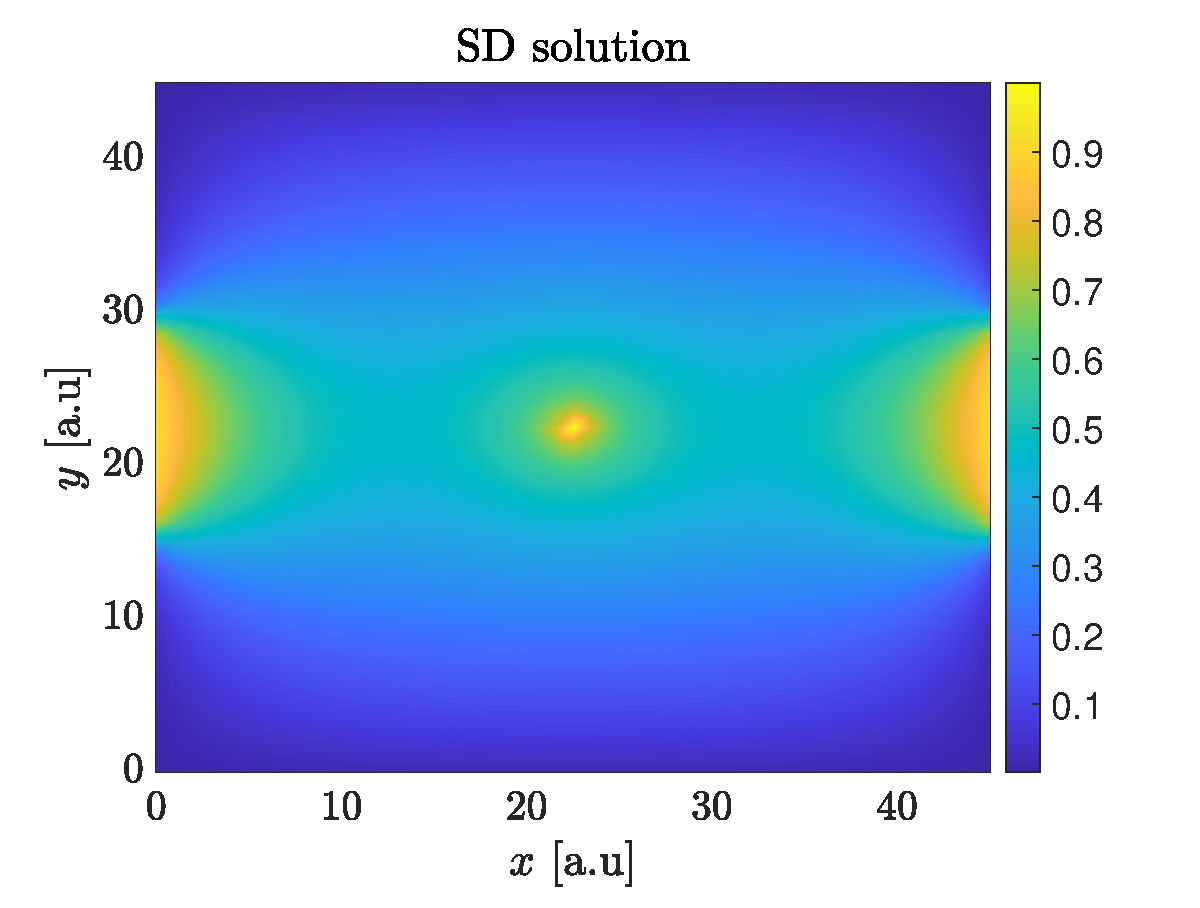
\includegraphics[scale=0.4]{SD_solution.eps} 
            \caption{}
            \label{SD_sol}
            \end{subfigure}
            \hfill
            \begin{subfigure}{0.48\textwidth}
            \includegraphics[scale=0.4]{CG_solution.eps}
            \caption{}
            \label{CG_sol}
            \end{subfigure}
            \caption{Left: Electric potential obtained by the SD algorithm - Right: Same for the CG algorithm}
\end{figure}

It was also possible to determine $N_{it}$ the number of iterations required to get to those solutions. In the case of the SD method, $7'890$ iterations were required to converge to a solution whose error w.r.t Matlab's solution is $3.5\cdot10^{-11}$. As of the CG method, only $239$ iterations were required. The error w.r.t Matlab's solution is $1.7\cdot10^{-15}$, which is not far from machine precision.\\

Note that the solutions obtained are physically consistent. Indeed, the obtained electric potential is 1V at the centre of the grid where a charge of 1C has been placed. Moreover, the electric field moves from areas of high electric potential (conductors) to areas of low electric potential (insulators), which is consistent with the laws of electromagnetism.\\

\end{homeworkSection}

\begin{homeworkSection}{(4) Jacobi preconditioning} 

The main idea of preconditioning is to solve the system $\bA \bx=\mathbf{b}$ indirectly, i.e. by solving $\mathbf{M}^{-1}\bA \mathbf{x}=\mathbf{M}^{-1}\mathbf{b}$. Different preconditioning can be implemented, such as the Jacobi preconditioning for example, where one defines the matrix $\mathbf{M}$ as diagonal, formed by the diagonal elements of $A$. As expected, the Jacobi preconditioning accelerated the convergence of the SD and CG methods. Indeed, the number of iterations required for the convergence were now $7'430$ iterations for the SD and  $220$  for the CG methods.\\

\end{homeworkSection}

\vspace{1cm}

\end{homeworkProblem}

 
%%%%%%%%%%%%%%%%%%%%%%%%%%%%%%%%%%%%%%%%%%%%%%%%
%%%%%%%%%%%%%%%%%%%%%%%%%%%%%%%%%%%%%%%%%%%%%%%%
\newpage

\begin{homeworkProblem}
\section{Nonlinear conjugate gradient method }

Consider an ensemble of $N$ identical atoms interacting with each other by means of a pair potential 
\begin{gather}\label{lennard jones energy}
    E(\bx_1,…,\bx_N)=\sum_{i\neq j}U_{LJ}(|\bx_i-\bx_j|)
\end{gather}
where $\{\bx_i\}$ are the coordinates of atoms and $U_{LJ}(\bx)$ is the Lennard-Jones potential which describes weak van der Waals interaction 
\begin{gather}\label{lennard jones potential}
    U_{LJ}(x)=4\epsilon\left[\left(\frac{\sigma}{x}\right)^{12}-\left(\frac{\sigma}{x}\right)^{6}\right]
\end{gather}
The minima on the potential energy surface described by $E(\bx_1,…,\bx_N)$ correspond to equilibrium configurations of Lennard-Jones potential. This potential is implemented in the file \verb|LennnardJones.m|.\\

\begin{homeworkSection}{(1) Algorithm} 

The methods previously used (SD and CG) were used to find the minima of a quadratic form in order to solve the associated linear problem. However, some physics situations require to solve more complicated problems, in the sense that they wouldn't necessarily be linear. That is a reason to introduce the non-linear conjugate gradient (NLCG) method.\\
 
\noindent This algorithm, implemented in the \verb|non_linCG.m| file, is  based on the CG algorithm, but different regarding what follows. A recursive formula in the residual calculation cannot be used. The residual is then constantly fixed at the opposite of the gradient, that is $r_i=-f'(x_i)$. Moreover, the $\beta$ coefficient is calculated thanks to Fletcher-Reeves formula, i.e. $\beta_{i+1}=r_{i+1}^tr_{i+1}/(r_i^tr_i)$. Finally, finding $\alpha$ the step size is somehow more complicated. To overcome this difficulty, a Newton-Raphson method is used. The main idea is to minimize, using a Taylor expansion of order 2, the expression $f( \bx+\alpha \mathbf{d})$ along the vector $\mathbf{d}$, as it has been shown in the lecture notes. In that problem, the functional to minimize, $f$, is the  energy $E$ as defined in Eq.(\ref{lennard jones energy}).\\

The Newton-Raphson method writes\\

\begin{gather}
    E(\bx+\alpha \mathbf{d})\sim E(\bx)+\alpha(E'(\bx))^t+\frac{\alpha^2}{2}\mathbf{d}^tE''(\bx)\mathbf{d}
\end{gather}\\

\noindent where $E''(\bx)$ is the Hessian matrix, containing the second order derivatives of E with respect to the coordinates. Note that it only needs to be evaluated in the direction $\mathbf{d}$ (see \verb|Hessian.m| file). Finally, when the second derivative is negative, the step is taken in the direction of the maximum rather than the minimum. Thus the idea is to take a small step of $-\epsilon E'(\mathbf{x})$ down the gradient.\\

\end{homeworkSection}

\subsubsection{Test of the algorithm}

In order to test NLCG algorithm, the cases of $N\in\{2,3\}$ have been implemented. For these two configurations, the equilibrium positions were determined thanks to the NLCG method (see Fig.(\ref{n=2}) and Fig.(\ref{n=3})). The total energy $E$ of the equilibrium configuration was also determined. These are given by $E_2=-1$ and $E_3=-3$.
\begin{figure}[H]
            \centering
            \begin{subfigure}{0.48\textwidth}
            \includegraphics[scale=0.21]{n=2.png} 
            \caption{}
            \label{n=2}
            \end{subfigure}
            \hfill
            \begin{subfigure}{0.48\textwidth}
            \includegraphics[scale=0.21]{n=3.png}
            \caption{}
            \label{n=3}
            \end{subfigure}
            \caption{Left: final configuration minimizing the energy functional in the case of 2 atoms - Right: same for 3 atoms}
\end{figure}


\noindent Those obtained equilibrium configuration seem to agree with the Lennard-Jones potential. Indeed, the term to the 6th power in Eq.(\ref{lennard jones potential}) accounts for the attraction between atoms and dominates at long distances, while the term to the 12th power is an empirical term that accounts for Pauli's exclusion principle. \\



\begin{homeworkSection}{(2) $N=4$} 
	
Consider now the case of a molecule of 4 atoms. Two distinct equilibrium configurations are possible:  the square planar geometry and the tetrahedral geometry (see \ref{n=4 tetra} and \ref{n=4 squared}, respectively).

\begin{figure}[H]
            \centering
            \begin{subfigure}{0.48\textwidth}
            \includegraphics[scale=0.205]{n=4_squared.png} 
            \caption{}
            \label{n=4 tetra}
            \end{subfigure}
            \hfill
            \begin{subfigure}{0.48\textwidth}
            \includegraphics[scale=0.205]{n=4_tetrahedral.png}
            \caption{}
            \label{n=4 squared}
            \end{subfigure}
            \caption{Equilibrium configurations in the case of 4 atoms.}
\end{figure}

\noindent In order to obtain the tetrahedral configuration, the atoms were initially disposed randomly. The total energy of the equilibrium configuration is negative and is $E_{4,t}=-6$. Since the energy is negative, this state is a stable equilibrium bound state. To recover the flat square equilibrium configuration, the initial positions must not be set randomly. In fact, the tetrahedral configuration is more stable than the planar square configuration, which is then favorable in the case of random initial positions. However, any rectangular or square initial configuration will converge to a plane square equilibrium configuration, whose total energy is $E_{4,s}=-4.4806$. Thus, the square equilibrium is also a stable bound state, but less stable than the tetrahedral configuration ($E_{4}^t<E_{4}^s$). 
\end{homeworkSection}



\begin{homeworkSection}{(3) $N=5$} 
The same analysis is now carried out on a system made up of 5 atoms. Clusters of 5 atoms can arrange either in trigonal bi-pyramid (see Fig.(\ref{n=5 pyramid})) or a square pyramid geometry (see  Fig.(\ref{n=5 trigo})).\\

\begin{figure}[H]
            \centering
            \begin{subfigure}{0.48\textwidth}
            \includegraphics[scale=0.22]{n=5_pyramid.png} 
            \caption{}
            \label{n=5 trigo}
            \end{subfigure}
            \hfill
            \begin{subfigure}{0.48\textwidth}
            \includegraphics[scale=0.22]{n=5_trigonal_bipyramid.png}
            \caption{}
            \label{n=5 pyramid}
            \end{subfigure}
            \caption{Left: quare pyramid equilibrium configuration ($N=5$ atoms) - Right: trigonal equilibrium}
\end{figure}

To obtain the previous equilibrium configurations, the same approach as for $N=4$ was used. A set of random positions is used to obtain a trigonal bi-pyramidal equilibrium. The total energy of this equilibrium configuration is $E_{5,t}=-9.1039$, characteristic of a stable bound state. To get the square pyramid equilibrium configuration, any configuration whose pyramidal base is flat and whose last atom is positioned along the axis perpendicular to the plane formed by the first 4 atoms converges towards a square pyramidal equilibrium configuration. A scan on various positions following that configuration has been made. In that case, the total energy of the system is given by $E_{5,s}=-8.4806$. Thus the square pyramid configuration also corresponds to a stable bound state. Note that this configuration can be considered less stable as the trigonal bi-pyramid configuration since $E_{5,t}<E_{5,s}$.\\
\end{homeworkSection}

\begin{homeworkSection}{(4) $N=6$} 

Increasing the number of atoms lead to more diverse equilibrium configurations. The first one is given by the trigonal prismatic geometry. This configuration is obtained by placing three atoms on the vertices of a triangle.For convergence speed purposes, the triangle was chosen to be equilateral. In addition, one atom is placed on a straight line perpendicular to the plane formed by the first 3 atoms. The last two atoms are placed on the opposite side of the plane formed by the first 3 atoms. The resulting equilibrium's energy is of  $E_{6,t}=-12.3029$. The equilibrium configuration is pictured in Fig.(\ref{n=6 trigonal})

\begin{figure}[H]
            \centering
            \begin{subfigure}{0.48\textwidth}
            \includegraphics[scale=0.22]{n=6.png} 
            \caption{}
            \label{n=6 trigonal}
            \end{subfigure}
            \hfill
            \begin{subfigure}{0.48\textwidth}
            \includegraphics[scale=0.22]{n=6_bipyramid.png}
            \caption{}
            \label{n=6 pyramid}
            \end{subfigure}
            \caption{Left: trigonal equilibrium configuration ($N=6$ atoms) - Right: bipyramid equilibrium}
\end{figure}

The second one considered here is the octahedral geometry. This configuration can be obtained by imposing a plane base of 4 atoms, square or rectangular, and placing the two remaining atoms on a straight line perpendicular to that plane, on either side of the latter (equally spaced or not). Fig.(\ref{n=6 pyramid}) shows this equilibrium configuration for a total energy of $E_{6,o}=-12.7121$. \\


\end{homeworkSection}





\vspace{1cm}

\end{homeworkProblem}


%%%%%%%%%%%%%%%%%%%%%%%%%%%%%%%%%%%%%%%%%%%%%%%%
%%%%%%%%%%%%%%%%%%%%%%%%%%%%%%%%%%%%%%%%%%%%%%%%
\newpage

\begin{homeworkProblem}

\section{SVD: Over-defined system of linear equations}

\begin{homeworkSection}{(1) SVD - method} 
	
The Singular Value Decomposition (SVD) consists in the decomposition of a real or complex matrix $\bA$ of size $m\times n$ ($m\ge n$) in the following product $\bA=\mathbf{U}\mathbf{\Sigma} \mathbf{V}^{\star}$, where $\mathbf{U}$ is a $m\times m$ unitary matrix of left-singular vectors, $\mathbf{V}$ is a $n \times n$ unitary matrix of right-singular vectors and  $\mathbf{\Sigma}$ is a $m \times n$ diagonal matrix of singular values. The SVD can be very useful to solve over-defined system of linear equations such as the one from Eq.(\ref{SVD_system}).\\

\beq
\left(\begin{array}{cc}  3 & 2  \\ 4 & 5  \\ 1 & 1 \end{array}\right)\left(\begin{array}{c} x_1 \\ x_2 \end{array}\right) = \left(\begin{array}{c} 1 \\ 4 \\ 1 \end{array}\right)\iff \bA \bx = \mathbf{b}. 
\label{SVD_system}
\eeq

\noindent Since the system is over-defined (in our case 3 equations for 2 unknowns), the idea is to minimize the residual $r$, defined as $r(\bx)=||\bA\bx-\mathbf{b}||$. If $A$ is a full-rank matrix, then the solution of the system of linear equation can be written as $\bx=\bA^{+}\mathbf{b}$, where $\bA^{+}$ denotes the Penrose inverse of the matrix $\bA$. The Penrose inverse of $\bA$ can be obtained running the Matlab command \verb|pinv(A)|. In that case, it yields the following result for $\bx^* := \bx$ such that  $r(\bx)$ is min: $\bx^* = (x^*_1,x^*_2) = (-0.4118, 1.1373)$.
	
	
\end{homeworkSection}

\begin{homeworkSection}{(2) SVD - example} 
We verify easily that the result given in \textbf{(1)} is correct by computing the residual in the plane $(x_1,x_2)$ around $(x^*_1,x^*_2) $. The solution obtained lies indeed at the minimum of the paraboloid formed by the contours of the residual, as depicted in Fig.(\ref{residual})

\begin{figure}[h!]
\centering
	\includegraphics[width = 0.5 \textwidth]{overdefined.png}
	\caption{\label{residual}  Contours of the residual $r(\bx)$ in the vicinity of $\bx^*$. The red $+$ marks the position of $\bx^*$}
\end{figure} 
\end{homeworkSection}

\end{homeworkProblem}



%%%%%%%%%%%%%%%%%%%%%%%%%%%%%%%%%%%%%%%%%%%%%%%%
%%%%%%%%%%%%%%%%%%%%%%%%%%%%%%%%%%%%%%%%%%%%%%%%

\newpage

\begin{homeworkProblem}

\section{SVD: Quantum state tomography}

\subsection{The density matrix formalism}

In order to describe quantum systems, it is of crucial importance to be able to express statistical distribution of quantum states. The density matrix formalism provides a tool for such a study. Let us consider a statistical mix of $N$ states $\ket{\psi_n}$, each with probability $p_n$ such that $\sum_n p_n=1$. The density matrix describing this mixture is defined as:\\

\begin{gather}\label{rho}
    \hat{\rho}=\sum_{n}p_n\ket{\psi_n}\bra{\psi_n}
\end{gather}\\

\begin{homeworkSection}{(1) Diagonalization}
 
The first part of this exercise deals with the diagonalization of the following density matrices:\\

\begin{gather}
    \hat{\rho_1}=\frac{1}{2}\begin{pmatrix}
        1&1\\
        1&1
    \end{pmatrix},\qquad
    \hat{\rho_2}=\frac{1}{2}\begin{pmatrix}
        -3&-1\\
        -1&1
    \end{pmatrix}
\end{gather}\\

\noindent Let us denote the resulting diagonal matrices by $D_1$ and $D_2$, respectively.\\

\begin{gather}
    D_1=\begin{pmatrix}
        0&0\\
        0&1
    \end{pmatrix},\qquad
    D_2=\begin{pmatrix}
        \frac{2+\sqrt{2}}{2}&0\\
        0&\frac{2-\sqrt{2}}{2}
    \end{pmatrix}
\end{gather}\\

\end{homeworkSection}

\noindent Recall that in quantum mechanics, the state of a system is described by an element $\ket{\psi}$ from the Hilbert space associated with the system. Such a state can be described by the density operator:\\
 
\begin{homeworkSection}{(2) Density matrix properties}
\begin{gather}
    \hat{\rho}=\ket{\psi}\bra{\psi}
\end{gather}\\

\noindent If a density operator is of this form, it satisfies  $\hat{\rho}^2=\hat{\rho}$. Conversely, if $\hat{\rho}^2=\hat{\rho}$, then there exists $\ket{\psi}$ such that $\hat{\rho}=\ket{\psi}\bra{\psi}.$ In that case, $\rho$ is said to describe a \textit{a pure state}. This result can be proven as follows. If $\hat{\rho}^2=\hat{\rho}$, then in the basis that diagonalizes $\hat{\rho}$, it comes that $\lambda_i=0$ or $1$. But $\sum_i\lambda_i=1$. Therefore, there exists $n$ such that $\lambda_n=1$ and $\lambda_j=0$ for $j\neq n$. This implies that $\hat{\rho}=\ket{\psi_n}\bra{\psi_n}$. Hence, the $\ket{\psi_n}$ state is the eigenvector of the density matrix associated with the non-zero $\lambda_n$ eigenvalue.\\

\noindent It can be verified that $\hat{\rho}_1^2=\hat{\rho}_1$. As a result, there is a state $\ket{\psi}$ such that $\hat{\rho}=\ket{\psi}\bra{\psi}$. This state is given by $\ket{\psi}=\frac{1}{\sqrt{2}}(\ket{+}+\ket{-})$, where $\ket{+}$ and $\ket{-}$ are the eigen-kets of $\hat{\sigma}_z$. \\

In addition, the density matrix has the following properties: $\hat{\rho}$ is Hermitian, with trace equal to 1. Therefore, not every $2\times2$ matrix can be a valid density matrix. However, considering the generic decomposition of a $2\times2$ matrix following: \\

\begin{gather}\label{rho pauli}
    \hat{\rho}=\sum_{n=0}^{3}\rho_n\hat{\sigma}_n
\end{gather}\\

\noindent where $\rho_n\in\mathbb{C}$, $\hat{\sigma}_{0}\equiv\hat{1}$ and $\hat{\sigma}_n$, $n\neq0$, are the Pauli matrices. Thus, constraints on $\rho_n$ can be established to ensure that the properties of a density matrix are satisfied. The matrix from Eq.(\ref{rho pauli}) can be calculated explicitly, giving \\

\begin{gather}\label{def coeff rho}
    \hat{\rho}=\begin{pmatrix}
        \rho_0+\rho_3&\rho_1-i\rho_2\\
        \rho_1+i\rho_2&\rho_0-\rho_3
    \end{pmatrix}
    \quad\Longrightarrow\quad
    \begin{cases}
        \Tr(\hat{\rho})=1\quad\Leftrightarrow\quad\rho_0=1/2\\
        \hat{\rho}^{\dag}=\hat{\rho}\quad\Leftrightarrow\quad \rho_1,\rho_2,\rho_3\in\mathbb{R}
    \end{cases}
\end{gather}\\

\end{homeworkSection}

\subsection{Simple Quantum state tomography}

\begin{homeworkSection}{(1) Density matrix reconstruction}

The goal of the quantum tomography is to reconstruct the density matrix $\hat{\rho}$. Generally, a single observable does not provide enough information to fully reconstruct the density matrix. To generalize this approach, let us consider $M/2$ observables, yielding $M$ projection operators defined as follows:\\

\begin{gather}\label{projecteurs}
    \hat{E}_m\equiv\ket{\psi_m}\bra{\psi_m}
\end{gather}\\

\noindent In a similar way, let $p_m$ be the probability associated with $\hat{E}_m$. Thus, the following system of equations $p_m=\Tr(\hat{\rho}\hat{E}_m)$, $m=1,...,M$, has to be solved. With the decomposition from Eq.(\ref{rho pauli}), this system of equations can be cast into a matrix equation according to $\mathbf{p}-\mathbf{M}_0=\mathbf{M}\mathbf{\rho}$, where\\
 
\begin{gather}\label{matrice de mesure}
    \mathbf{p}=(p_1,…,p_M)^T,\quad \mathbf{M}_0=(1/2,...,1/2)^t,\quad\mathbf{\rho}=(\rho_1,\rho_2,\rho_3)^T,\quad (\mathbf{M})_{m,i}=\Tr(\hat{\sigma}_i\hat{E}_m),\,i\in\{1,2,3\}
\end{gather}\\

\noindent The matrix $\mathbf{M}$ is the so-called \textit{measurement matrix}. Using the Penrose inverse (\verb|pinv| command in Matlab) and the basis formed by the $\ket{n\pm}$ vectors, i.e. the eigenvectors of the $\hat{\sigma}_n$ operator, it is possible to reconstruct the density matrix for a given probability vector $\mathbf{p}$. These vectors are given by the files \verb|p1.csv| and \verb|p2.csv|. Note that by convention, $\ket{\psi_{1,2}}=\ket{x\pm}$, $\ket{\psi_{3,4}}=\ket{y\pm}$ and $\ket{\psi_{5,6}}=\ket{z\pm}$. The matrix $\mathbf{M}$ was constructed using the matlab function from  \verb|measurement.m|. Solving the equation $\mathbf{p}-\mathbf{M}_0=\mathbf{M}\mathbf{\rho}$ using the Penrose inverse, which is possible since the rank of $M$ is 3, gives the following $\mathbf{\rho}$s vectors, associated with the probability vectors $\mathbf{p}_1$ and $\mathbf{p}_2$, respectively\\
 
\begin{gather}\label{rho1 et rho2}
    \vec\rho_1=\begin{pmatrix}
        0.3536\\
        0\\
        0.3536
    \end{pmatrix},\qquad
    \vec\rho_2=\begin{pmatrix}
        0.2439\\
        0.3\\
        0.2707
    \end{pmatrix}
\end{gather}\\

\noindent Finally, combining Eq.(\ref{rho pauli}) and Eq.(\ref{rho1 et rho2}), it follows that the reconstructed density matrices are:\\
 
\begin{gather}\label{new rho1 rho2}
    \hat{\rho}_1=
    \begin{pmatrix}
        0.8536&0.3536\\
        0.3536&0.1464
    \end{pmatrix},\qquad
    \hat{\rho}_2=
    \begin{pmatrix}
        0.7707&0.2439-0.3i\\
        0.2439+0.3i&0.2293
    \end{pmatrix}
\end{gather}\\

\noindent One can be observe that for both $\hat{\rho}_1$ and $\hat{\rho}_2$, $\Tr(\hat{\rho}_i)=1$, $i\in\{1,2\}$. Moreover, $\hat{\rho}_i=\hat{\rho}^{\dag}_i$ is satisfied. In addition, it can also be verified that $\hat{\rho}_1^2=\hat{\rho}_1$, but $\hat{\rho}_2^2\neq\hat{\rho}_2$. Thus, there is a state $\ket{\phi}$, such that $\hat{\rho}_1=\ket{\phi}\bra{\phi}$. This state is given by the eigenvector of $\hat{\rho}_1$ associated to its non-zero eigenvalue:\\
 
\begin{gather}
    \ket{\phi}=
    \begin{pmatrix}
        -0.9239\\
        -0.3827
    \end{pmatrix}
\end{gather}\\
\end{homeworkSection}

\begin{homeworkSection}{(2) Reconstruction with less projection operators}
The same analysis was carried out, but this time only with the first 4 projection operators, i.e. $\ket{\psi_{1,2}}=\ket{x\pm}$ and $\ket{\psi_{3,4}}=\ket{y\pm}$. In this case, 
the singular values of the measurement matrix are given by $\sigma_1=\sqrt{2}$, $\sigma_2=\sqrt{2}$ and $\sigma_3=0$. As a result, the $M$ measurement matrix is not full-rank. In other words, the matrix $M$ is singular, and the Penrose inverse cannot be used to solve the equation $\vec p-\vec M_0=M\vec\rho$.\\

\end{homeworkSection}


\subsection{Quantum state tomography with experimental constraints}

\begin{homeworkSection}{(1) Reconstruct the density matrix? }

Experimentally, it can happen that the measurement can only be performed along a direction specified by two angles $\theta$ and $\phi$, yielding:\\

\begin{gather}
    \ket{\psi(\theta,\phi)}\equiv
    \begin{pmatrix}
        \cos\theta/2\\
        e^{i\phi}\sin\theta/2
    \end{pmatrix}.
\end{gather}\\

\noindent The projection operator is, as before, defined by $\hat{E}=\ket{\psi(\theta,\phi)}\bra{\psi(\theta,\phi)}$. However, a single observable is not enough to reconstruct the density matrix. Thus, let us consider a single fermion subject to an external magnetic field along the $\hat{z}$ direction. Assuming that the Hamiltonian $\hat{H}$ is given by $\hat{H}=\hbar\Omega\hat{\sigma_z}$, with $\Omega$ the angular frequency of the magnetic field, it can be shown that \\

\begin{gather}
    e^{i\hat{H}t/\hbar}\ket{\psi(\theta,\phi)}=\ket{\psi(\theta,\phi-\Omega t)}
\end{gather}\\

\noindent In other words, measuring at different times is equivalent to rotating the axis. This rotation allows to gain a lot more information about the system, but is not guaranteed to be sufficient to fully reconstruct the density matrix.\\

\noindent The first step is to determine by mean of SVD, whether or not reconstruction of the density matrix is possible. To this end, various properties of the SVD will be exploited, in particular the fact that the number of non-zero singular values represents the rank of the considered matrix. This information will enable to determine if the matrix is full rank or not. \\

To that end, let us consider the following set of projection operators : $\ket{\psi(\theta,\phi_m)}\bra{\psi(\theta,\phi_m)}$, where $\phi_m=2\pi k/M$, $k=0,...,M-1$. This is equivalent to a measurement along the $(\theta,\phi=0)$ axis, for $M$ different times, uniformly distributed between $t=0$ and $t=2\pi/\Omega$. The SVD was carried out on the measurement matrix (see Eq.(\ref{matrice de mesure})) for $\theta\in\{0,\pi/2,\pi/3\}$ and $M=100$. The singular values obtained have been arranged in a vector $\vec v_{\theta_i}$ to make it easier to read. The index $\theta_i$ corresponds to the angle $\theta$ considered. \\

\begin{gather}
    \vec v_{0}=\begin{pmatrix}
        10\\
        0\\
        0
    \end{pmatrix},\quad
    \vec v_{\pi/2}=\begin{pmatrix}
        7.1063\\
        7.0356\\
        2.08\cdot10^{-15}
    \end{pmatrix},\quad
    \vec v_{\pi/3}=\begin{pmatrix}
        6.1554\\
        6.0930\\
        4.99
    \end{pmatrix}
\end{gather}\\

\noindent It can therefore be concluded that the density matrix can only be reconstructed here when $\theta=\pi/3$. Indeed, in the case where $\theta=0$, it is clear that there are zero singular values. In the case where $\theta=\pi/2$, the singular value of the order of $10^{-15}$ is of the order of the machine precision and is therefore considered zero. Recalling that the number of non-zero singular values corresponds to the rank of the matrix (the measurement matrix in this case), when $\theta=\pi/3$, the measurement matrix is full-rank. The Penrose inverse can then be used to solve $\mathbf{p}- \mathbf{M}_0=\mathbf{M}\mathbf{\rho}$ and reconstruct the density matrix according to Eq.(\ref{rho pauli}).  \\
\end{homeworkSection}

\begin{homeworkSection}{(2) New measurements}
A new collection of $M=200$ measurements was carried out. Note that this time $\theta=5\pi/7$ and that $\mathbf{p}$ was recovered from \verb|ps3.csv|. The vector of singular values is given by \\

\begin{gather}
    \vec v_{5\pi/7}=\begin{pmatrix}
        8.8183\\
        7.8369\\
        7.7987
    \end{pmatrix}
\end{gather}\\

\noindent Therefore the measurement matrix is full rank. The $\rho_i$, $i\in\{1,2,3\}$, coefficients used to reconstruct the density matrix according to Eq.(\ref{rho pauli}) are given by:\\

\begin{gather}
    \vec\rho=
    \begin{pmatrix}
        0.2555\\
        -0.0705\\
        0.2385
    \end{pmatrix}
    \quad \Longrightarrow \quad \hat{\rho}=
    \begin{pmatrix}
        0.7385&0.2555+0.0705i\\
        0.2555-0.0705i&0.2615
    \end{pmatrix}
\end{gather}\\

\end{homeworkSection}

\begin{homeworkSection}{(3) EWV}
It can be checked that the $\hat{\rho}$ matrix obtained is a valid density matrix. Indeed, $\Tr(\hat{\rho})=1$ and $\hat{\rho}=\hat{\rho}^{\dag}$. However, measurements of probabilities $\mathbf{p}$ are experimental, so there are uncertainties $\Delta \mathbf{p}$ associated with them. These uncertainties will propagate to yield an uncertainty on the reconstructed density matrix. To assess the robustness of the previous tomography procedure, the \textit{equally weighted variance} (EWV) is used\\

\begin{gather}
    EWV=\sum_{n=1}^{3}\sum_{m=1}^{M}(M_{nm}^+)^2(\Delta p_m)^2
\end{gather}\\

\noindent where $\mathbf{M}^+$ is the Penrose inverse of the measurement matrix $\mathbf{M}$. Note that the subscript $M$ in the sum corresponds to the number of measurements made ($M=2001$ in this case) and should not be confused with the measurement matrix $M$. The uncertainty of the $M$ measurements made in this experiment is estimated as $\Delta p_m=0.1+0.001(m-1)$. Fig.(\ref{EWV}) shows the evolution of the quantity EWV as a function of $\theta$, where $\theta\in[0,\pi]$.\\

\begin{figure}[H]
    \centering
    \includegraphics[scale=0.5]{EWV.png}
    \caption{Evolution of EWV as a function of $\theta$, with $\theta\in[0,\pi]$.}
    \label{EWV}
\end{figure}

Thus, the minima seem to be in $\theta\in\{0,\pi/2,\pi\}.$ However, it should be noted that for these values, the $\mathbf{M}$ matrix is singular. As a result, the density matrix cannot be reconstructed from these $\theta$ values. Nevertheless, the value of $\theta\approx1.0477$ also represents a local minimum, for which $\mathbf{M}$ does not have a zero singular value. As a result, the value of $\theta$ which minimises the uncertainty $\Delta\mathbf{p}$ and allows the density matrix to be reconstructed is $\theta\approx\pi/3$.\\
	
\end{homeworkSection}

\end{homeworkProblem}
%%%%%%%%%%%%%%%%%%%%%%%%%%%%%%%%%%%%%%%%%%%%%%%%
%%%%%%%%%%%%%%%%%%%%%%%%%%%%%%%%%%%%%%%%%%%%%%%%






\end{spacing}

\newpage
\bibliographystyle{alpha}
\bibliography{references}
\end{document}
\end{document}

%%%%%%%%%%%%%%%%%%%%%%%%%%%%%%%%%%%%%%%%%%%%%%%%%%%%%%%%%%%%%
